% Gibt die Klasse des Dokuments an
\documentclass[a4paper]{scrartcl}
% passende Kodierung fĂĽr deutsche Sonderzeichen
%\usepackage[T1]{fontenc}
% bequemer Eingabezeichensatz(fĂĽr Eszett etc.)
\usepackage[utf8]{inputenc}
% FĂĽr align-Umgebung etc.
\usepackage{amsmath, amsthm}
% For graphics
\usepackage[pdftex]{graphicx}


% deutsche Silbentrennung/Rechtschreibung
%\usepackage[ngerman]{babel}
\usepackage{amssymb}


% Eigene Befehle
\newtheorem{thm}{Theorem}[section]
\newtheorem{cor}[thm]{Korollar}
\newtheorem{defi}[thm]{Definition}
\newtheorem{lem}[thm]{Lemma}
\newtheorem{bem}[thm]{Bemerkung}

% Standardmengen
\newcommand{\R}{\mathbb{R}}
\newcommand{\Q}{\mathbb{Q}}
\newcommand{\Z}{\mathbb{Z}}
\newcommand{\N}{\mathbb{N}}
\newcommand{\E}{\mathbb{E}}
\newcommand{\rainf}{\rightarrow \infty}



\begin{document}
% Title
\title{Classification with Restricted Boltzmann Machines}
\author{Katarzyna Tarnowska \and Fritjof Wolf}
\maketitle

% Abstract
\begin{abstract}
\textbf{Abstract:}
The aim of the project was to implement Restricted Boltzmann Machines as classifier and examine what effect different parameters have on the performance. Chosen classification problem was character/image recognition. The implementation was trained using Contrastive Divergence learning algorithm and tested on the MNIST and CIFAR-10 datasets. 
\end{abstract}
\newpage

% Textbody
\section{Introduction}
% some general remarks about topic, what we do and the different sections


\section{Restricted Boltzmann Machines}
\begin{center}
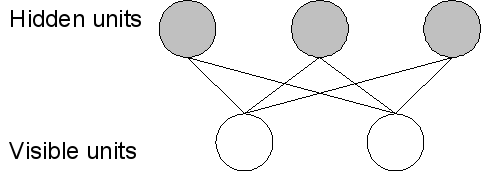
\includegraphics[width=4cm]{images/rbm.png}
\captionof{figure}{The Restricted Boltzmann Machine architecture. Source: \cite{Krizhevsky}  }
\end{center} 
...
Hinton \cite{Hinton} describes three approaches to using Restricted Boltzmann Machines for classification:
\begin{itemize}
    \item Using the hidden features learned by the RBM as the inputs for some standard discriminative method
    \item Training a separate RBM on each class
	\item Training a joint density model using a single RBM
\end{itemize}
The first method is a powerful and promising approach especially when several RBMs are stacked such that the input of the n-th RBM is the output of the (n-1)-th RBM in order to learn more abstract features. These so-called Deep Belief Networks have been widely studied in the both theory and practice, see e.g. (\cite{DeepBelief}), but will not be further discussed in this report. The remainder will focus on the last two methods, which are an at the same time both simple and effective way to use RBMs for classfication. 

\subsection{Models}
\paragraph{Generative RBM}
\begin{center}
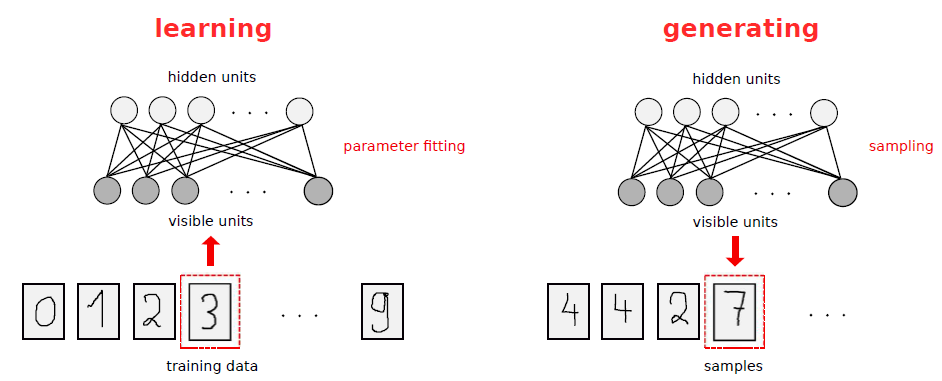
\includegraphics[width=12cm]{images/generativeRBM.png}
\captionof{figure}{Generative model of RBM. Source: \cite{Fischer} }
\end{center}
\paragraph{Discriminative RBM}
Joint density model assumes that RBM has two sets of visible units. Besides the units representing a data vector ({\bfseries x}), there are units representing a label - {\bfseries y}. Label is therefore expressed by binary indicator variables, one of which is set to 1, indicating a particular label (for the case of handwritten images - a particular digit), while the others are set to 0. 
As a result of two sets of visible units, there are also two sets of weights: between data and hidden units ({\bfseries W}) and between label units and hidden units ({\bfseries U}). 
\begin{center}
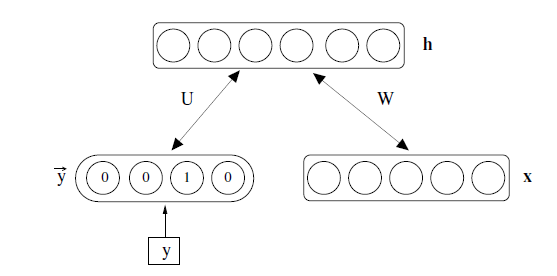
\includegraphics[width=8cm]{images/jointProbModel2.png}
\captionof{figure}{Joint probability model of Restricted Boltzmann Machines. Source: \cite{Larochelle}}  
\end{center}
Model learns joint probability distribution with n-step contrastive divergence (CD) algorithm (reconstruction step is performed n-times before updating weights). Training is performed on mini-batches of the training set. In terms of the CD algorithm, it means that weights are updated after estimating a gradient on a subset of training cases (a "mini-batch"), instead of on a one single training case. Such approach is known to be more efficient and enabling computation parallelism by means of multi-threading and multi-core systems.
\begin{center}
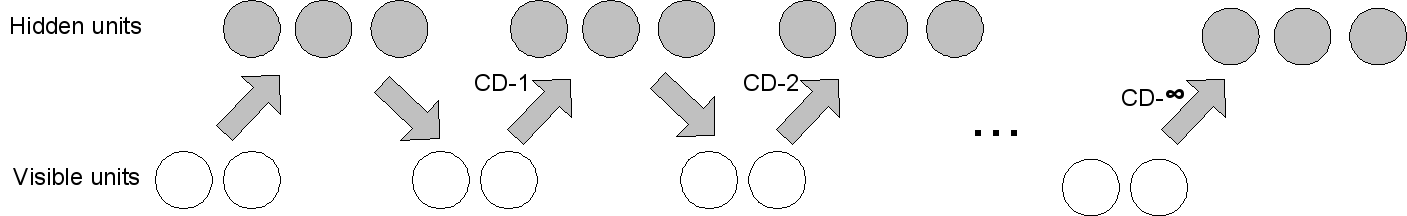
\includegraphics[width=12cm]{images/cd-n.png}
\captionof{figure}{Illustration of n-step contrastive divergence learning algorithm. Source: \cite{Krizhevsky}}  
\end{center} 
\par Class prediction is done by choosing the most likely label given the input, under the learned model. In more detail, it fixes the visible units corresponding to the test data input and samples target units, with the use of learned weights. In the last sampling iteration the target units are set to probabilities values instead of stochastic binary units. The predicted class is the position in the binary vector with the highest probability. 
\begin{center}
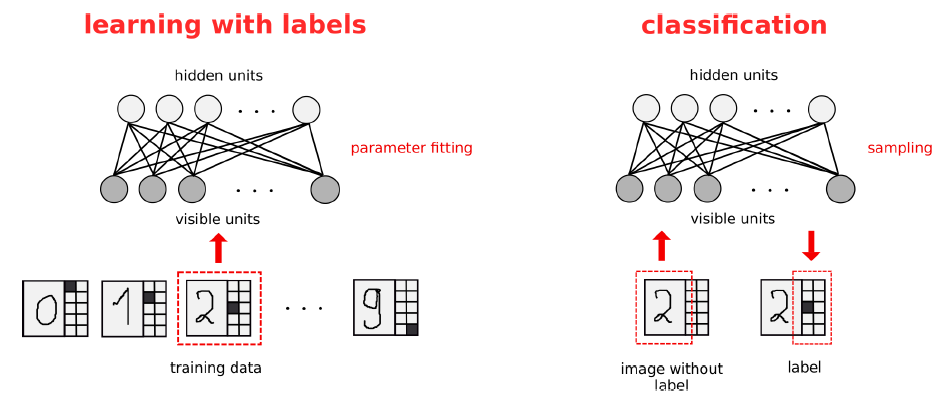
\includegraphics[width=12cm]{images/DRBM.png}
\captionof{figure}{Classification with discriminative model of RBM. Source: \cite{Fischer} }
\end{center}
Another approach for class prediction is based on computation of free energy \cite{Hinton}. After training, a test vector is tried with each label, and the one that gives lowest free energy is chosen as the most likely class ('test-against-all-labels' prediction approach for DRBM).

\subsection{The MNIST Dataset}
\begin{minipage}[t]{0.5\textwidth}
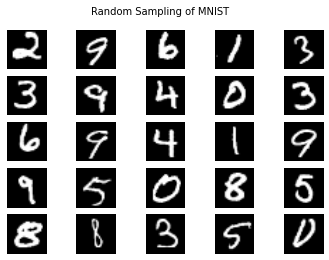
\includegraphics[width=7cm]{images/mnist-example.png}
\captionof{figure}{Examples from the MNIST dataset, source: \cite{mnist-example}}
\end{minipage}
\par The main dataset used in the experiments was MNIST dataset of handwritten digit images. The dataset is widely used for training and testing in the field of machine learning. The images are 28 x 28 pixels, and the dataset is divided into 60,000 training cases and 10,000 test cases. The training set is further divided into a training set of 50,000 cases and a validation set of 10,000 cases. The validation set is used to perform model selection and hyper-parameter selection, whereas the test set is used to evaluate the final generalization error and compare different algorithms in an unbiased way.
\paragraph{Preprocessing} For greyscale digit images, pixel values can be interpreted as degrees of blackness on a white background. To make data binary, the pixel intensities (0-255) were scaled (to values between 0 and 1) and then binarized with threshold of 0.5. Another possible way to make data binary is to treat the pixel intensities as probabilities and sample from the given Bernoulli distribution for each pixel. 
\par It is also possible to reduce dimensionality by downsizing the size of images - for example to 8x8 (for faster training times). Another preprocessing technique - data 'nudging' can generate several times bigger data by 'shifting' images (perturbing the data with linear shifts of 1 pixel in each direction). This way it is possible to learn decent representations from a smaller dataset.
 
 
 
\section{Empirical Results for Discriminative RBM}
This section describes the empirical results of a RBM trained with joint density model (the third approach of using RBM's for discrimination, described by Hinton \cite{Hinton}).
\par The first aim of testing implemented RBM was finding optimal hyper-parameters (optimal model parameters). The choice of optimal hyper-parameters was based on the observation of reconstruction error convergence. It was not possible to perform computational-intensive cross-validation or grid search for optimal hyper-parameters taking into account long training times. The preliminary experiments were done on the smaller datasets- trainset of 100 cases in 100-epoch training. Times measured on PC Intel Pentium Dual CPU T3200 @2GHz, RAM 3 GB with CPU mean usage about 0.75 and memory mean usage about 2,3GB.
\subsection{Monitoring progress of learning}
As it is easy to compute the squared error between the data and the reconstructions, this quantity is often a good indicator of a progress of learning \cite{Hinton}. Within experiments on training the RBM, mean squared error was printed out after each epoch. It enabled the observation of the general progress or characteristic of learning as well as any abnormalities and potential problems in hyperparameter settings. 
While MSE is quite good and simple indicator of progress of learning, it is not the function that $CD_n$ is optimizing. The better indicator of what is happening during learning are graphic displays of learned filters. Plotted weights of each unit as a gray-scale image after different numbers of epochs are shown on figures below. Such filters highlight strong features in the data.
\begin{minipage}[t]{0.5\textwidth}
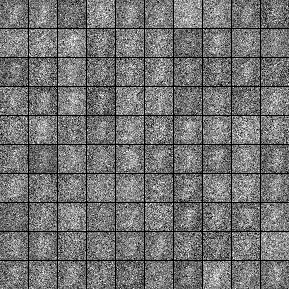
\includegraphics[width=7cm]{images/filtry_1epoch_50train.png}
\captionof{figure}{Learned filters after 1. epoch \newline of training}
\end{minipage}
\begin{minipage}[t]{0.5\textwidth}
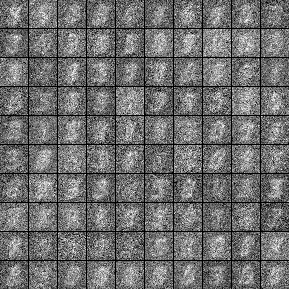
\includegraphics[width=7cm]{images/filtry_5epoch_50train.png}
\captionof{figure}{Learned filters after 5. epoch \newline of training}
\end{minipage}
\begin{minipage}[t]{0.5\textwidth}
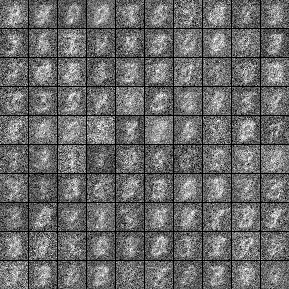
\includegraphics[width=7cm]{images/filtry_10epoch_50train.png}
\captionof{figure}{Learned filters after 10. epoch \newline of training}
\end{minipage}
\begin{minipage}[t]{0.5\textwidth}
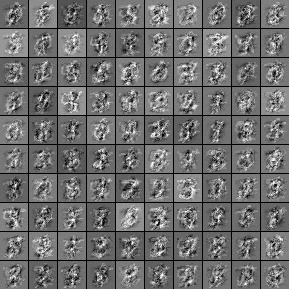
\includegraphics[width=7cm]{images/filters_epoch500_train50.png}
\captionof{figure}{Learned filters after 500. epoch \newline of training}
\end{minipage}

\subsection{The learning rate}
\par The results from training RBM with different learning rates are shown on the figure below.
\begin{center}
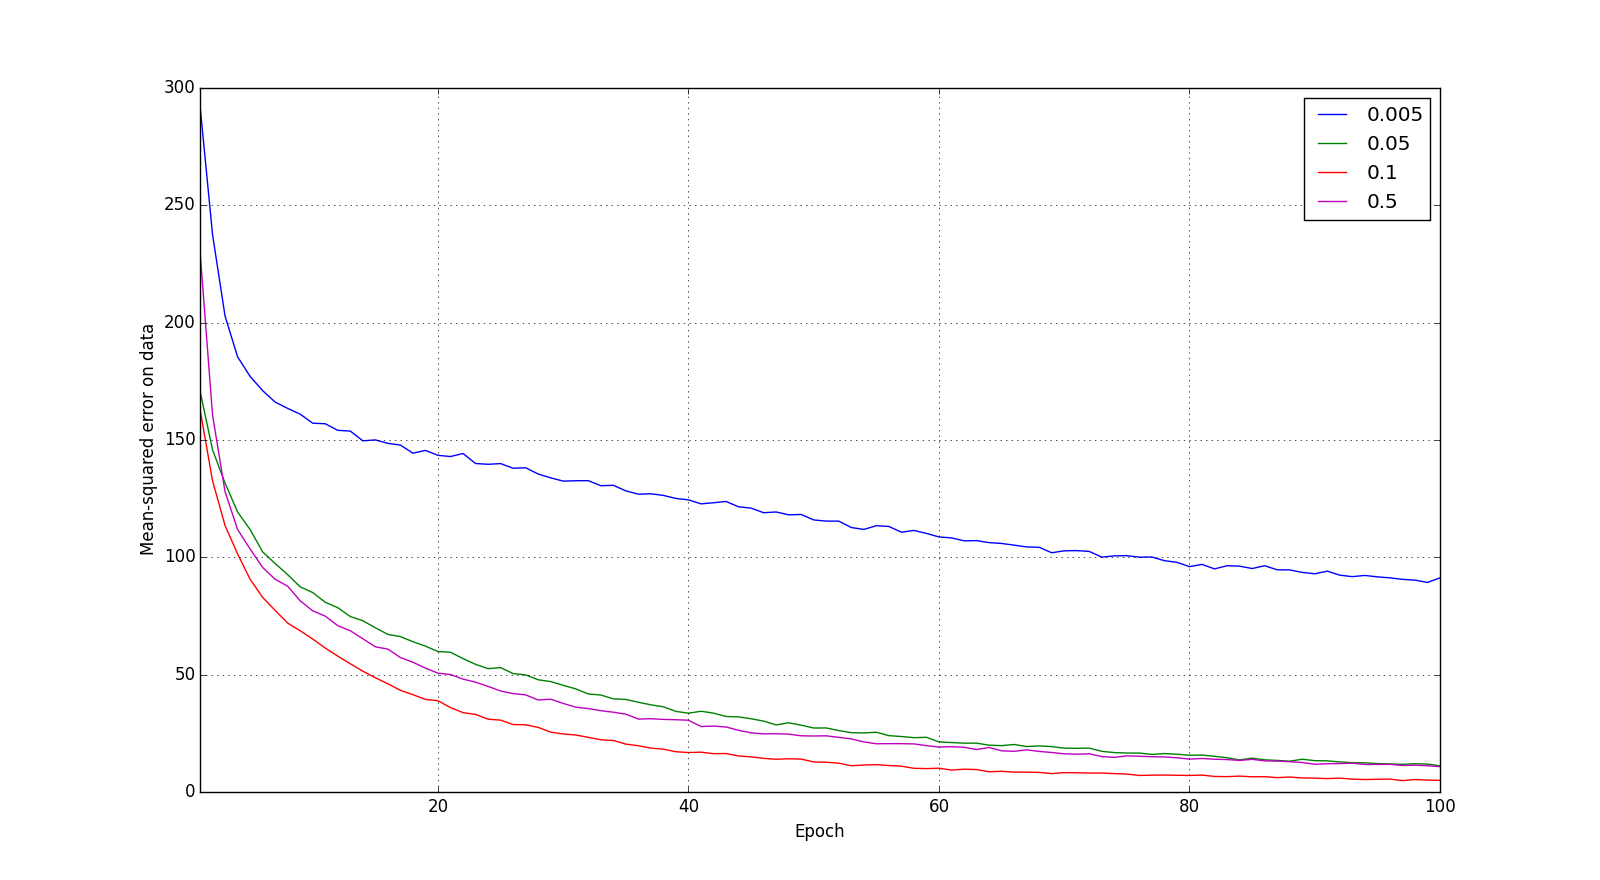
\includegraphics[width=14cm]{images/lr.png}
\captionof{figure}{Convergence comparison for different learning rates.}  
\end{center}
Learning rate of a magnitude between $10^{-2}$ and $10^{-3}$ seems to be optimal. The exact optimal magnitude depends also on the training data size, as tests on larger data sizes have shown (for example for smaller data sizes 0.1 was optimal, while for original sizes of 60000 learning rate of 0.01 was optimal). Additionally, too high learning rate (too high in relation to data size) caused instability and resulted in the reconstruction error increase (which is explained by Hinton \cite{Hinton} as a 'weight explosion'). 
\par Some research \cite{Tieleman} show that the learning rates used in experiments should not be constant and that in practice, decaying learning rates often work better. Experiment was done with varied learning rate, based on results from previous experiment and convergence observation for different learning rates: starting from 0.1, after 60. epoch decreased by half to 0.05, and after 80. epoch further decreased by an order of magnitude to 0.005. The varied learning rate model was compared with fixed learning rate model. The results are shown on the chart below.
\begin{center}
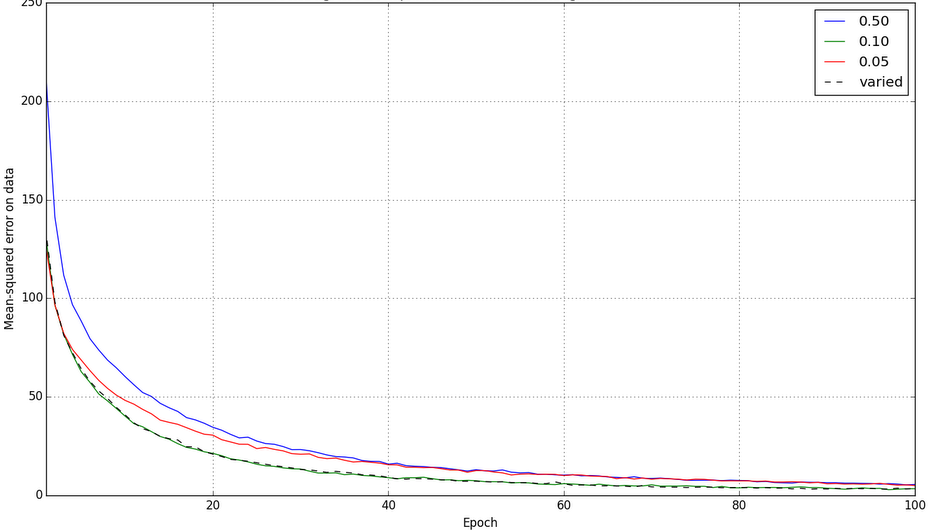
\includegraphics[width=14cm]{images/lr_var.png}
\captionof{figure}{Convergence comparison for different learning rates, including varied.}  
\end{center}
As it can be observed, decaying learning rate in a way described above does not change the reconstruction error convergence in comparison with the fixed learning rate model with value set to starting learning rate in varied model (dotted line almost overlap with the green one).
\subsection{The number of hidden units}
\par The second test was done on the number of hidden units. As figure below shows, the higher the number of hidden units, the better convergence of reconstruction error. On the other hand, greater hidden layer size causes longer training time (table).
\begin{center}
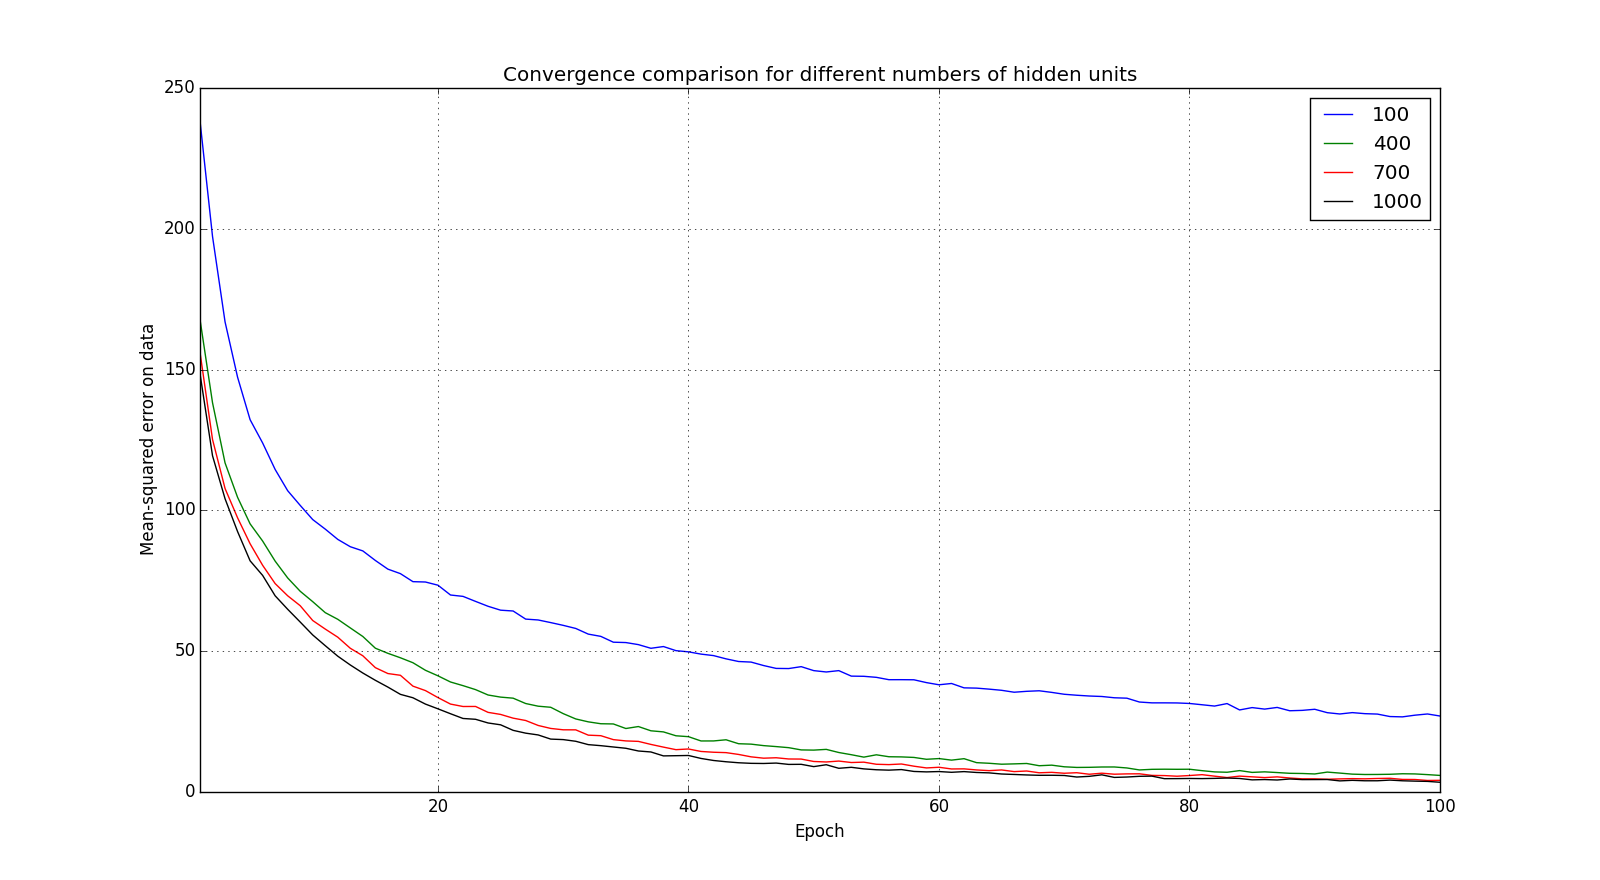
\includegraphics[width=14cm]{images/hu.png}
\captionof{figure}{Covergence comparison for different number of hidden units}  
\end{center}

\hspace{1cm}
\begin{tabular}{ | l || c | c | c | c | } 
	\hline
	Hidden units & 100 & 400 & 700 & 1000 \\ \hline
	Train time & 149.494s & 440.963s & 750.945s & 7658.844s \\ \hline
	MSE after 100 epochs & 26.981 & 5.887 & 4.149 & 3.457\\ 
	\hline 
\end{tabular}
\captionof{table}{Reconstruction error and train time comparison for different number of hidden units.} 
\subsection{The size of a mini batch}
The mini-batch optimization procedure should use only a small number of training points for each gradient estimate: 1,5,10. Higher mini-batch sizes (such as half of training set - 50) results in relatively high reconstruction error (figure below). 
\begin{center}
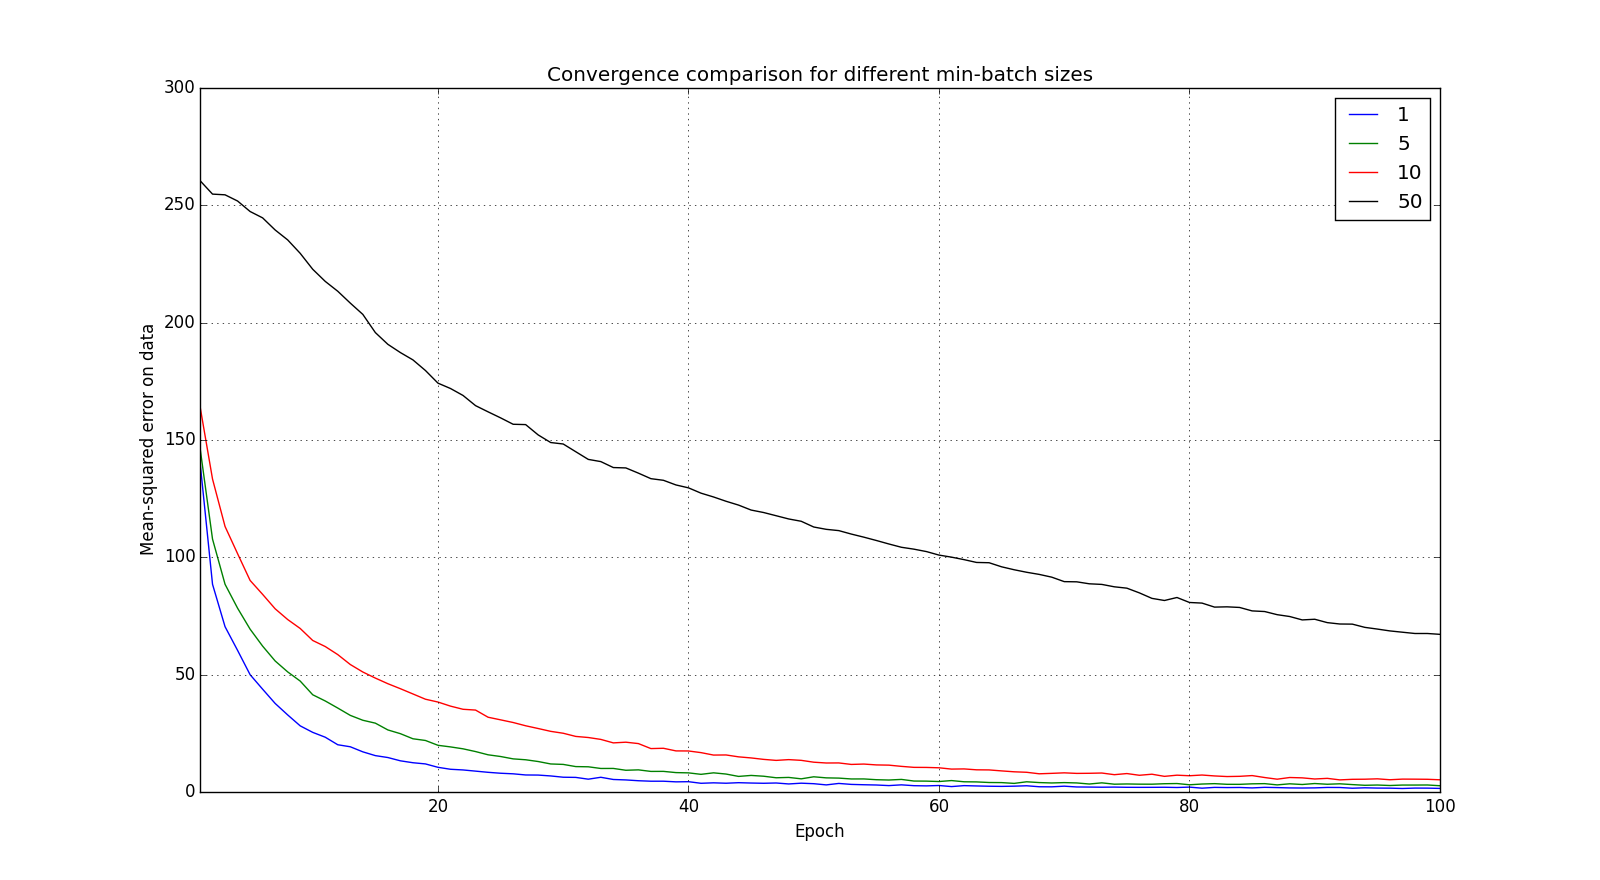
\includegraphics[width=14cm]{images/batch.png}
\captionof{figure}{Covergence comparison for different sizes of "mini-batches"}  
\end{center}
\hspace{1cm}
\begin{tabular}{|l||c|c|c|c|} \hline
Mini-batch size & 1 & 5 & 10 & 50
\\ \hline
Train time & 1137.937s & 618.903s & 578.186s & 514.207s
\\ \hline
MSE after 100 epochs & 1.526 & 2.669 & 5.202 & 67.182
\\ \hline \end{tabular}
\captionof{table}{Train time and MSE comparison for different sizes of "mini-batch".} 
\vspace{1cm}
Moreover, tests on classification accuracies on 50,000 training cases and 10,000 new cases have shown that size of ten (that is equal to the number of classes) seems to be optimal (see subsection 'Classification'). The ideal case for a mini-batch would be that each sample in it would represent a different class. In other words, each mini-batch should contain one example of each class to reduce the sampling error when estimating the gradient for the whole training set from a single mini-batch \cite{Hinton}. It is possible for datasets that contain a small number of equiprobable classes. However, for the MNIST dataset, the number of samples per each class is different. Therefore it is not possible to divide the data in such a way and preserve the original size of the dataset at the same time. On the other hand MNIST dataset was already randomized, so the samples are not sorted according to the class. Randomizing a dataset along with using minibatches of size about 10 (as advised in \cite{Hinton}) seems to work optimal in terms of classification error.
\subsection{The initial values of the weights and biases}
The weights are typically initialized to small random values chosen from a zero-mean Gaussian with a standard deviation of about 0.01. Test on initial weights with different initializations showed (see figure) that standard deviation of 0.1 features somehow better reconstruction error reduction that 0.01 and weights initialized to zeros (in each case biases are initialized with zeros).
All test runs were instantiated with a random number generator with fixed seed. Comparing continous and dotted lines of the same color on the chart below shows that changing the seed does not change the convergence significantly.
\begin{center}
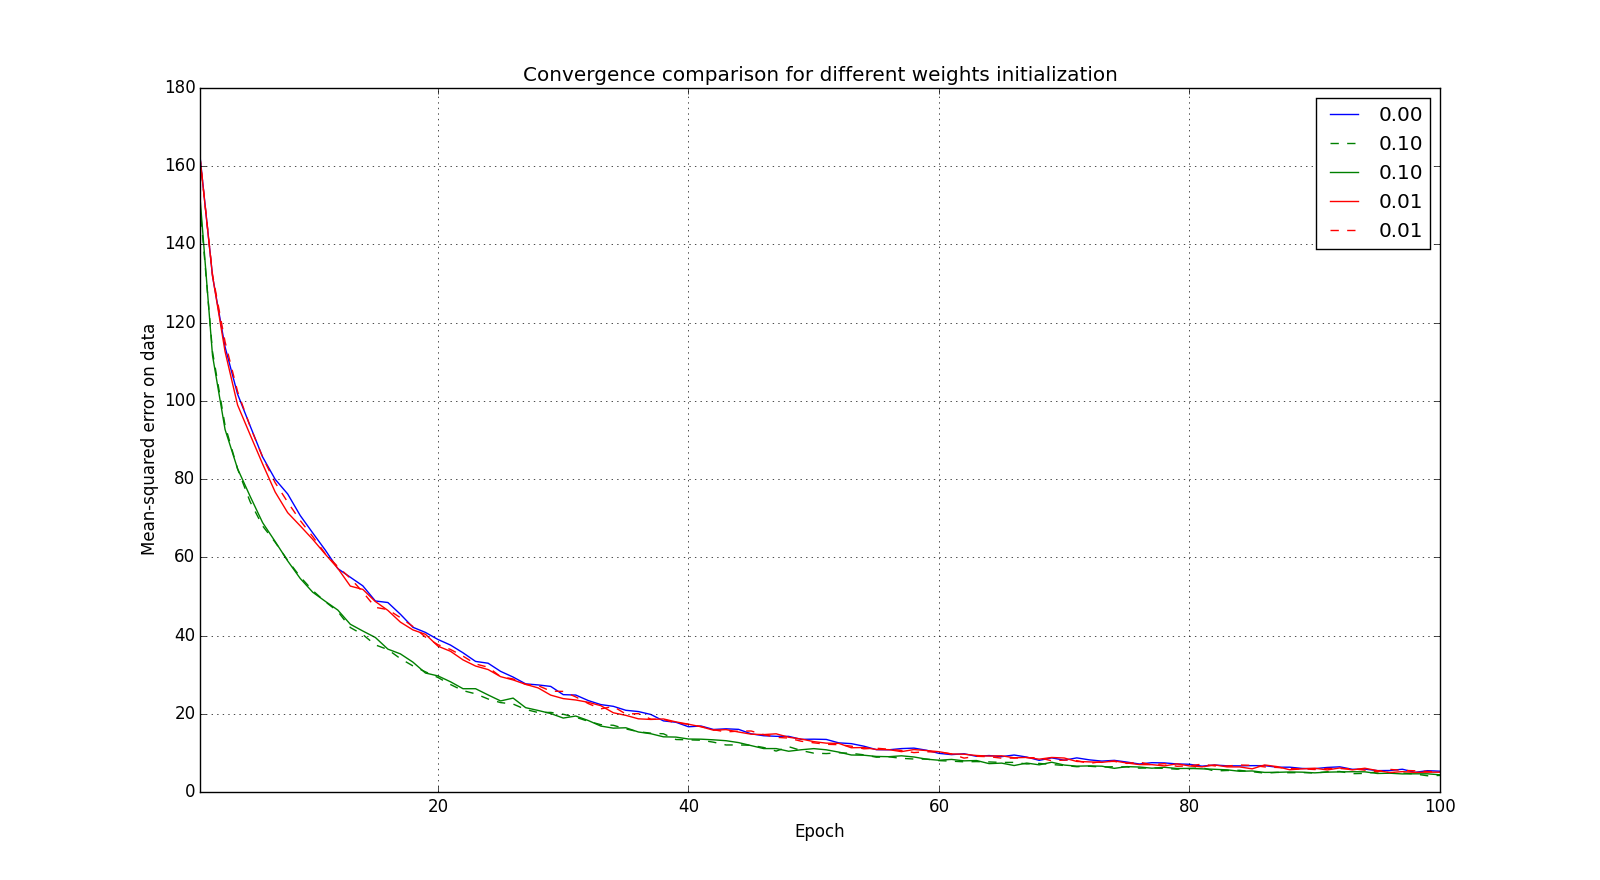
\includegraphics[width=14cm]{images/weights_seeds.png}
\captionof{figure}{Covergence comparison for different initializations of weights.}  
\end{center}
Chart below compares two models (blue and green lines) different in standard deviation of Gaussian, from which small random numbers are chosen for initial weight and bias values. It can be observed that for both cases changing initial biases from small random numbers to zeros does not affect the convergence of reconstruction error (dotted line almost overlap with continuous lines). It also shows that in case biases are not set to zero, it is better to use Gaussian with standard deviation of 0.01 rather than 0.1
\begin{center}
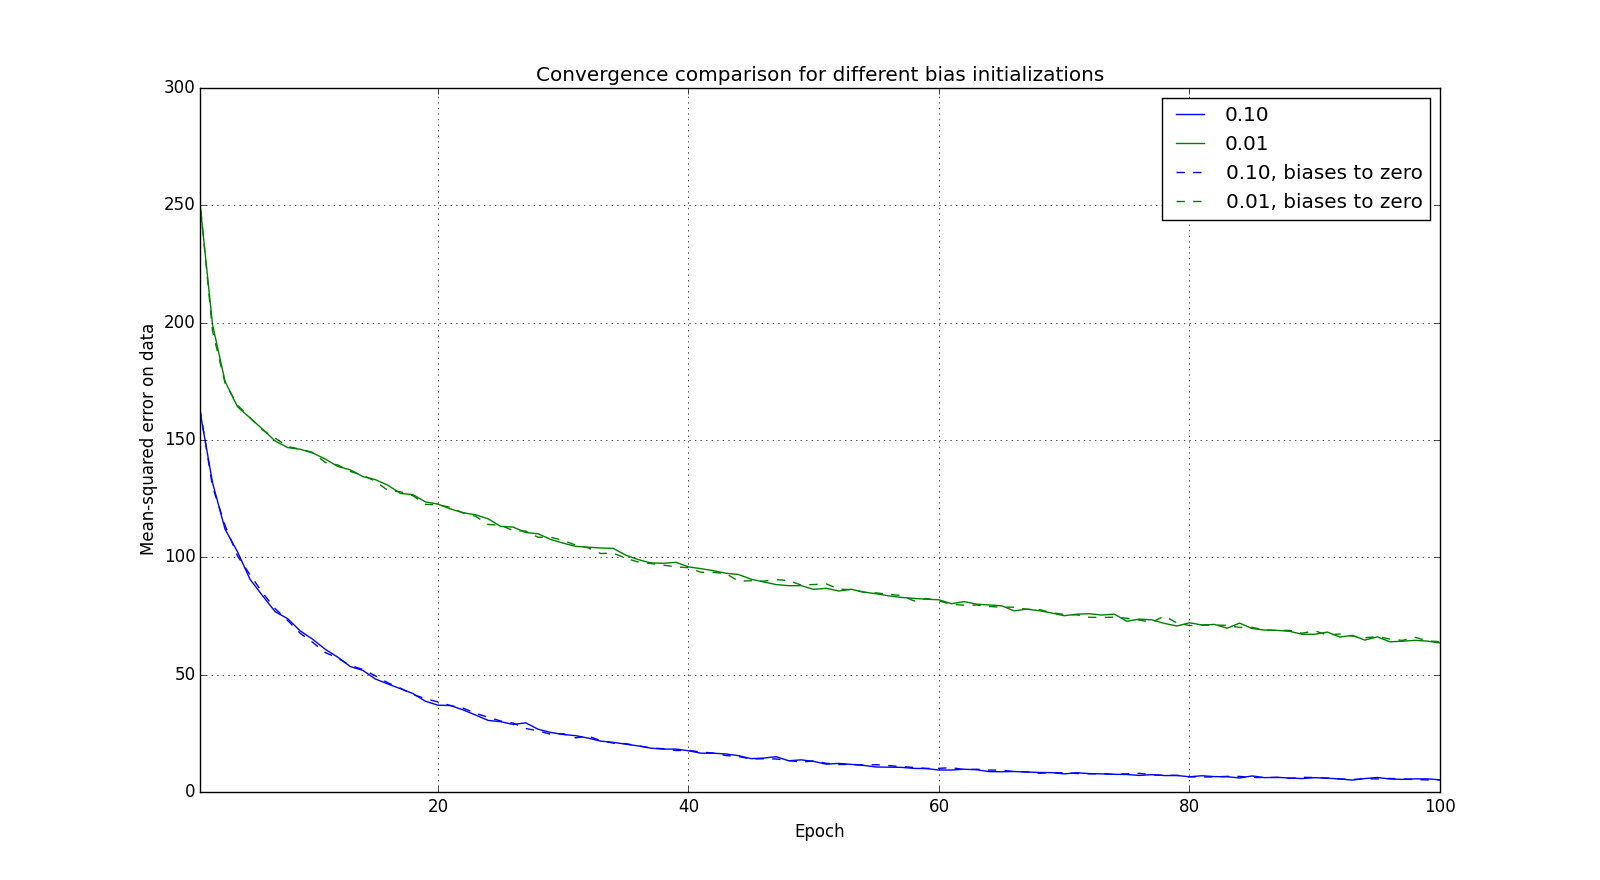
\includegraphics[width=14cm]{images/bias.png}
\captionof{figure}{Covergence comparison for different initializations of biases.}  
\end{center}

\subsection{Momentum}
Momentum is a simple method for increasing the speed of learning \cite{Hinton}. The "momentum" meta-parameter is the fraction of the previous velocity that remains after computing the gradient on a new mini-batch. The momentum method causes the parameters to move in a direction that is not the direction of steepest descent, so it could be regarded as the temporal smoothing method. It is advised \cite{Hinton} to start with a momentum of 0.5 and once the initial progress in the reduction of the reconstruction error settles down, increase it to 0.9. 
\begin{center}
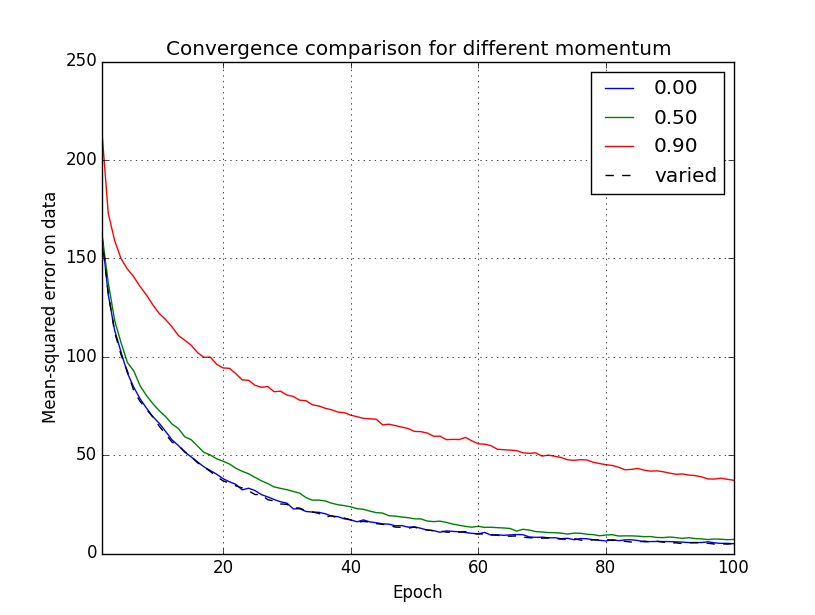
\includegraphics[width=14cm]{images/momentum_var.png}
\captionof{figure}{Covergence comparison for different momentum values.}  
\end{center}
The basic test on three momentum values: 0, 0.5 and 0.9 showed that the best convergence and the smallest reconstruction error is reached with momentum equal to zero. It also confirms that at least at the beginning of the training it is better to use lower value of momentum and possibly increase it while reduction in reconstruction error settles down. It could also be observed that increasing momentum while learning resulted in less oscillations in learning than in fixed model (compare dotted line on the figure with the blue one).

\subsection{Varieties of contrastive divergence}
$CD_1$ at the beginning of learning, when weights are small and mixing is fast, provides a good approximation to maximum likelihood. However, as weights grow, it makes sense to gradually increase the k in $CD_k$.
Figure shows that all models of $CD_1$, $CD_2$, $CD_3$, and varied model (with increasing k from 1 to 2 in 60. and to 3 in 80. epoch of training) seem to be converging to the similar value. Therefore, taking into account performance issues (higher number of contrastive divergence steps means longer training time - see table), it is sufficient to use one-step contrastive divergence algorithm.
\begin{center}
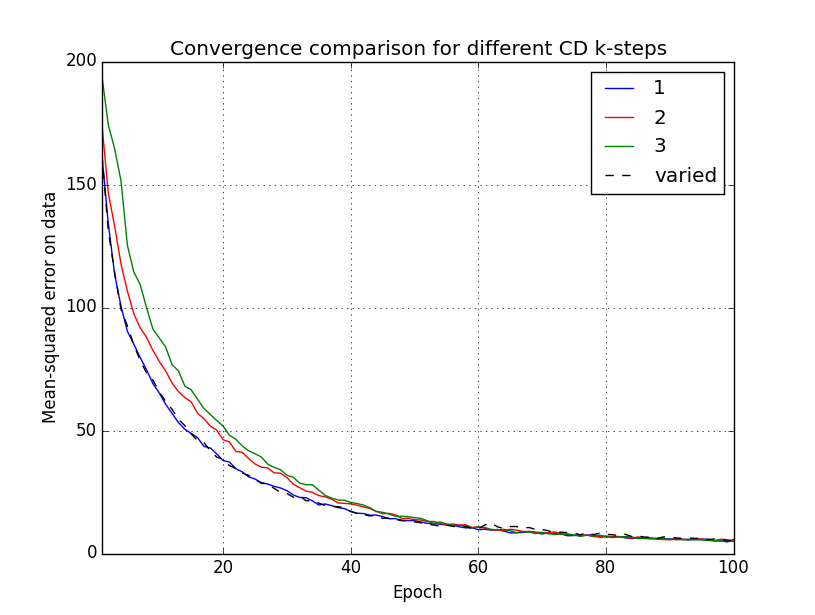
\includegraphics[width=14cm]{images/CDk_var.png}
\captionof{figure}{Covergence comparison for different contrastive divergence steps.}  
\end{center}
\hspace{1cm}
\begin{tabular}{|l||c|c|c|c|} \hline
k-step CD & $CD_1$ & $CD_2$ & $CD_3$ & $Varied$
\\ \hline
Train time & 551.038s & 783.783s & 968.845s & 616.180s
\\ \hline
MSE after 100 epochs & 5.631 & 4.965 & 4.912 & 5.607
\\ \hline \end{tabular}
\captionof{table}{Train time and MSE comparison for different numbers of contrastive divergence steps.} 

\subsection{Reconstruction}
After training process and choice of an optimal model, RBM can be used to show how well it reconstructs the data. Images below show a sample original image and reconstructed data. The reconstruction error after 500 epoch training falls below 1.0.
% first column
\begin{minipage}[t]{0.5\textwidth}
\begin{center}
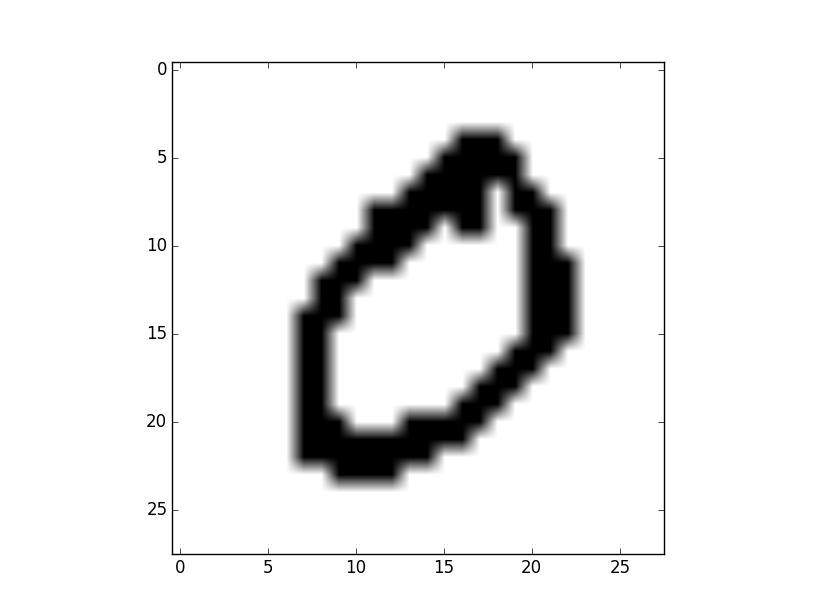
\includegraphics[width=4cm]{images/0original.png}
\captionof{figure}{Original image.}
\end{center}
\end{minipage}
\begin{minipage}[t]{0.5\textwidth}
\begin{center}
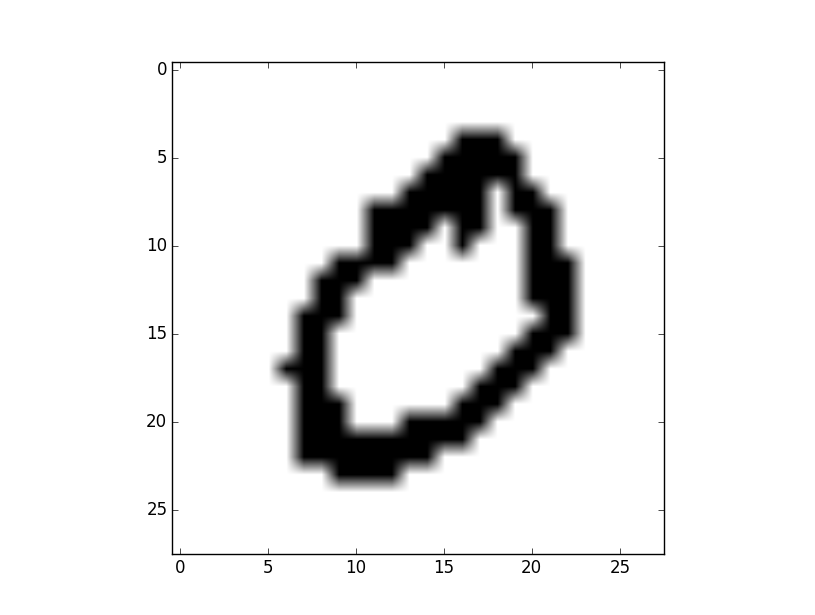
\includegraphics[width=4cm]{images/0_reconstructed_momentum00.png}
\captionof{figure}{Image reconstructed after training in 500 epochs.} 
\end{center}
\end{minipage}
\subsection{Classification}
After tests on model training and hyper-parameters choice, confronting them with best practices described in \cite{Hinton} RBM models were evaluated with classification metrics on the chosen MNIST dataset. The most important metric for classification task is accuracy, that is, the percentage of correct predictions. Second important metric for accuracy evaluation is confusion matrix, which informs which labels are mixed most often. Other metrics relevant to classification problem include: precision, recall and f1-score. The precision is the ratio tp / (tp + fp) where tp is the number of true positives and fp the number of false positives. The precision is intuitively the ability of the classifier not to label as positive a sample that is negative. The recall is the ratio tp / (tp + fn) where tp is the number of true positives and fn the number of false negatives. The recall is intuitively the ability of the classifier to find all the positive samples. The F1 score can be interpreted as a weighted average of the precision and recall, where an F1 score reaches its best value at 1 and worst score at 0. The formula for the F1 score is: \newline 
F1 = 2 * (precision * recall) / (precision + recall)
\par Example of classification metrics and confusion matrix are shown on the figures below. The training was performed on 10,000 cases in 100 epochs and testing on 1,000 new cases.
\begin{center}
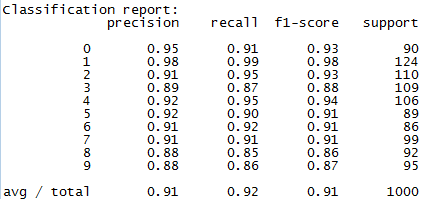
\includegraphics[width=10cm]{images/class_metrics.png}
\captionof{figure}{Example of classification report with precision, recall and f1-score for each digit class. Class of '1' performs best.} 
\end{center}
\begin{center}
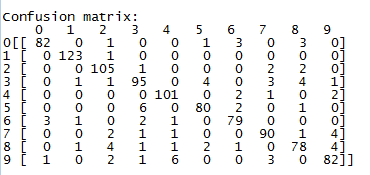
\includegraphics[width=8cm]{images/conf_matrix.png}
\captionof{figure}{Example of confusion matrix. $C_{i, j}$ is equal to the number of observations known to be in group i but predicted to be in group j. Shows which classes were mixed most often - '3' with '5' and '4' with '9'} 
\end{center}
\par Accuracy was computed by comparing the label predicted by RBM classifier with the original label on unseen data. Wrong predictions were counted and saved as images along with true and predicted labels. 
\paragraph{Method of samling target units} For the preliminary results, prediction method with target units sampling was used (see first section for method description). Table below shows classification accuracy obtained with this method on 50,000 dataset used for training and 10,000 validation set for computing accuracy. The table shows also main hyper-parameters chosen for training the model.
\begin{center}
\hspace{1cm}
\begin{tabular}{|l||c|c|c|c|} \hline
Accuracy & Learning rate & Hidden units & Training epoch & Batch Size
\\ \hline
95,2\% & 0.01 & 1000 & 100 & 10
\\ \hline
94,9\% & 0.01 & 2000 & 100 & 10
\\ \hline
94,8\% & 0.01 & 700 & 100 & 10
\\ \hline
94,0\% & 0.01 & 700 & 100 & 50
\\ \hline
93,1\% & 0.01 & 500 & 100 & 10
\\ \hline
92,7\% & 0.01 & 700 & 100 & 5
\\ \hline
92,7\% & 0.005 & 500 & 300 & 10
\\ \hline \end{tabular}
\captionof{table}{Classification accuracies with corresponding hyperparameters for RBM model training. Training performed on MNIST 50,000 set, classification on 10,000 validation data. Classification approach is based on sampling target units.}
\end{center}

The main obstacle in testing classification accuracy with different parameters were long times of training (on personal computers training and testing on original-size MNIST dataset took days to complete one run). Yet, the models with optimal parameters can be saved for further use.
\paragraph{Method based on free energy} In the next step, a prediction approach based on free energy computation was tested. Times and accuracy scores were compared with previous approach. This method proved to be incomparably faster and yielded better accuracy results. Instead of performing thousands of sampling iterations for each test vector it basically computes one value (free energy) against each label vector in turn. Therefore, using free energy-based approach is much more beneficial, when the classification problem is confined to small number of classes. 

\subsection{Different types of unit - Gaussian visible units}
RBMs are known to extract features more efficiently on binary data, than on the grayscale data. Experiments conducted on gaussian visible units (binarization step of scaled data was omitted) showed that they perform only slightly worse and basically comparably to models with binary units in terms of classification error(89,4\% versus 89,8\% on model trained on 3,000 cases in 100 epochs, tested on 1,000 test data). It was also observed that reconstruction error convergence of gaussian model is better than model with binary units (see linear chart), but seemingly it does not result in better classification performance. As training and prediction time are also comparable it can be concluded that gaussian values can be used for RBM model as well as binary ones. 

\begin{minipage}[t]{0.5\textwidth}

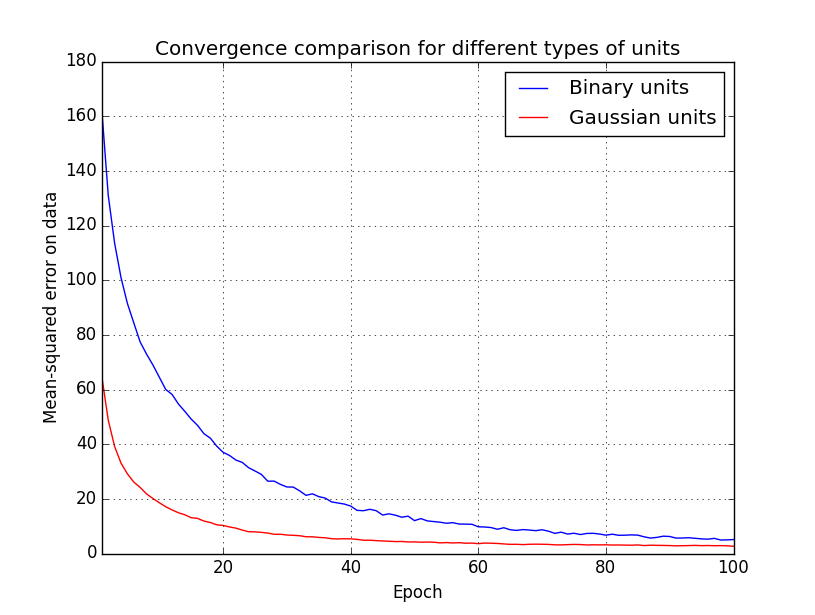
\includegraphics[width=7cm]{images/dataTypes.png}
\captionof{figure}{Reconstruction error convergence comparison between model with gaussian and binary units.} 

\end{minipage}
\begin{minipage}[t]{0.5\textwidth}

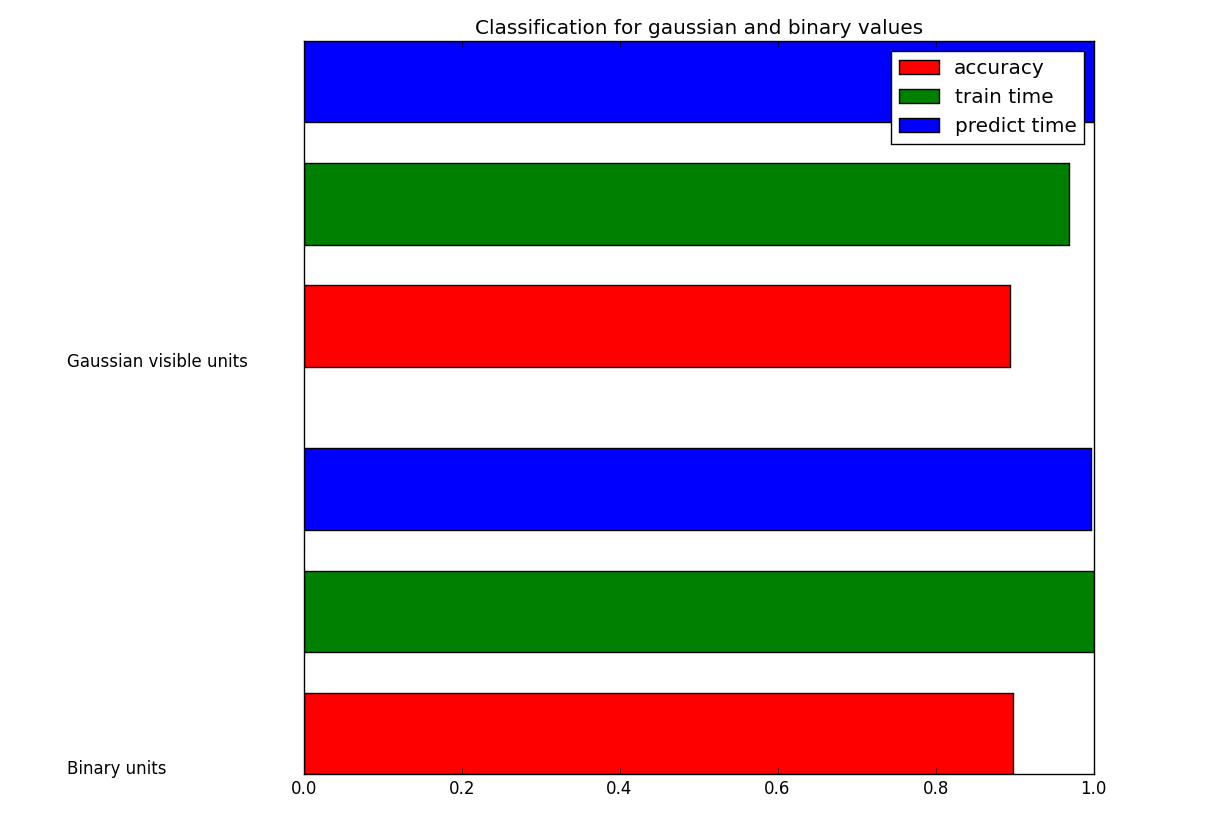
\includegraphics[width=8cm]{images/gaussian_binary.png}
\captionof{figure}{Classification comparison between models with different data types.}

\end{minipage}




\section{Empirical Results for the CIFAR dataset}

\subsection{The CIFAR Dataset}
\begin{center}
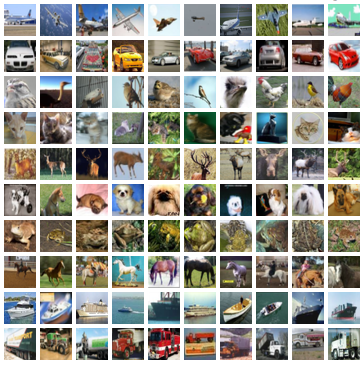
\includegraphics[width=4cm]{images/cifar-10.png}
\captionof{figure}{Examples from the CIFAR dataset Source: \cite{cifar-example}  }
\end{center} 


\section{Discussion}
Restricted Boltzmann Machines are often used as feature extractors or as an initialization step for deep belief networks. They were also successfully used as standalone classifiers. Recent research, such as described in paper \cite{Schmah}, show that both generative and discriminative versions of RBM classification, outperform other 'traditional' classifiers on real-world data. Moreover, discriminative versions of RBMs integrate discovering features of inputs with their use in classification, without relying on a separate classifier, facilitating model selection \cite{Larochelle}. Unsupervised learning (feature discovery) will remain a crucial component in building successful learning algorithms for AI on the grounds of scarcity of labeled examples and availability of many unlabeled. For the second, once a good high-level representation is learned, other learning tasks (e.g., supervised or reinforcement learning) could be much easier \cite{Bengio}. 
\par On the other hand, training RBM on a given dataset requires some practical experience in deciding how to set the values of hyper-parameters such as the learning rate, the momentum, the initial values of weights, the number of hidden units and the size of each mini-batch. It is also useful to know how to monitor the progress of learning and when to terminate the training. There exist no hard guidelines on what decisions should be made in all these aspects. In practice these decisions for each new application are often based on heuristics or trial-and-error approach. 
\par RBM's were developed using binary visible and hidden units, but other types of unit (gaussian, binomial) can also be used. This is important in dealing with data that is not well-modeled by binary visible units. 
\par Future work on classification with RBM may include implementing a Discriminative RBM as described in \cite{Larochelle}. The model optimizes directly $p(y \vert x)$ instead of merely p(x,y). The exact gradient can be computed efficiently and then used in a stochastic gradient descent optimization. As results on MNIST dataset in \cite{Larochelle} show, this model outperforms RBM modeling joint probabilities, with classification error 1.81\% versus 3.39\% . Further improvement on classification error was observed with Hybrid RBM (1.28\% ), described in the same paper.




% Literature
\begin{thebibliography}{9}
   \bibitem[1]{Krizhevsky} Krizhevsky, A. (2009) \emph{Learning multiple layers of features 	from Tiny Images} (Master thesis, Dept. of Comp.Sci., University of Toronto)
   \bibitem[2]{Hinton} Hinton, G. (2010) \emph{A Pratical Guide to Training Restricted 			Boltzmann Machines.} (UTML TR 2010-003)
   \bibitem[3]{Fischer} Fischer, A., Igel, Ch. (2008) \emph{Training Restricted Boltzmann 		Machines: An Introduction.} 
   \bibitem[4]{Larochelle} Larochelle H., Bengio, Y. (2008) \emph {Classification using 			Discriminative Restricted Boltzmann Machines} (Proceedings of the 25th International 			Conference on Machine Learning)
   \bibitem[5]{Schmah} Schmah T.,Hinton G., Zemel R., Small S. (2008) \emph{Generative 			versus discriminative training of RBMs
	for classification of fMRI images} (Conference on Advances in Neural Information 				Processing Systems 21)
   \bibitem[6]{Bengio} Bengio Y. (2009) \emph {Learning Deep Architectures for AI} 				(Foundations and Trends in Machine Learning
	Vol. 2, No. 1 )
   \bibitem[7]{Tieleman} Tieleman, T. (2008) \emph{Training Restricted Boltzmann Machines 		using Approximations to
	the Likelihood Gradient} (ICML 2008)	
   \bibitem[8]{DeepBelief} Hinton G., Osindero S., Yee-Whye T. \emph {A fast learning 			algorithm for deep belief nets}
   \bibitem[9]{mnist-example} http://andrew.gibiansky.com/blog/machine-learning/k-nearest-		neighbors-simplest-machine-learning/images/mnist-example-ipy.png
   \bibitem[10]{cifar-example} https://kaggle2.blob.core.windows.net/competitions/kaggle/3649/media/cifar-10.png
\end{thebibliography}


\end{document}
